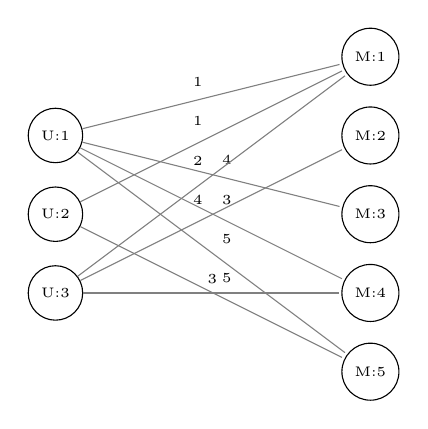
\begin{tikzpicture}[shorten >=1pt, auto, node distance=1cm, ultra thick]
\tikzstyle{node_style} = [circle,draw=black, thin, font=\tiny]
\tikzstyle{edge_style} = [draw=gray, line width=2, thin, font=\tiny ]

\node[node_style] (v1) at (-2,1) {U:1};
\node[node_style] (v2) at (-2,0) {U:2};
\node[node_style] (v3) at (-2,-1) {U:3};

\node[node_style] (v4) at (2,2) {M:1};
\node[node_style] (v5) at (2,1) {M:2};
\node[node_style] (v6) at (2,0) {M:3};
\node[node_style] (v7) at (2,-1) {M:4};
\node[node_style] (v8) at (2,-2) {M:5};

\draw[edge_style]  (v1) edge node{1} (v4);
\draw[edge_style]  (v1) edge node{4} (v6);
\draw[edge_style]  (v1) edge node{3} (v7);
\draw[edge_style]  (v1) edge node{5} (v8);
\draw[edge_style]  (v2) edge node{1} (v4);

\draw[edge_style]  (v2) edge node{5} (v8);
\draw[edge_style]  (v3) edge node{2} (v4);
\draw[edge_style]  (v3) edge node{4} (v5);
\draw[edge_style]  (v3) edge node{3} (v7);
\end{tikzpicture}